% Generated by paper/figures.py from results/. Do not edit.
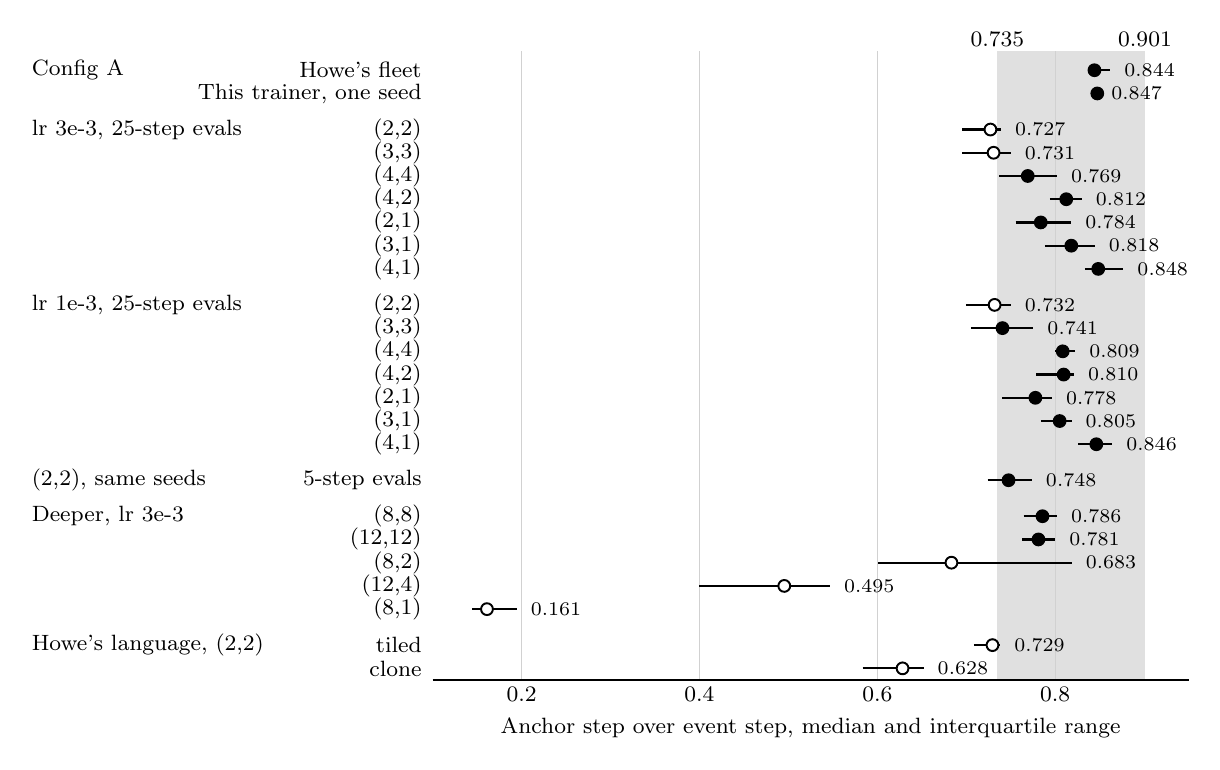
\begin{tikzpicture}
\fill[black!12] (12.322,0) rectangle (14.197,7.991);
\draw[black!18, line width=0.4pt] (6.279,0.000) -- (6.279,7.991);
\node[anchor=north, inner sep=1.5pt, align=left, font=\footnotesize] at (6.279,-0.030) {0.2};
\draw[black!18, line width=0.4pt] (8.538,0.000) -- (8.538,7.991);
\node[anchor=north, inner sep=1.5pt, align=left, font=\footnotesize] at (8.538,-0.030) {0.4};
\draw[black!18, line width=0.4pt] (10.797,0.000) -- (10.797,7.991);
\node[anchor=north, inner sep=1.5pt, align=left, font=\footnotesize] at (10.797,-0.030) {0.6};
\draw[black!18, line width=0.4pt] (13.056,0.000) -- (13.056,7.991);
\node[anchor=north, inner sep=1.5pt, align=left, font=\footnotesize] at (13.056,-0.030) {0.8};
\draw[black, line width=0.5pt] (5.150,0.000) -- (14.750,0.000);
\node[anchor=north, inner sep=1.5pt, align=left, font=\footnotesize] at (9.950,-0.420) {Anchor step over event step, median and interquartile range};
\node[anchor=south, inner sep=1.5pt, align=left, font=\footnotesize] at (12.322,7.991) {0.735};
\node[anchor=south, inner sep=1.5pt, align=left, font=\footnotesize] at (14.197,7.991) {0.901};
\node[anchor=west, inner sep=1.5pt, align=left, font=\footnotesize] at (0.000,7.744) {Config A};
\node[anchor=east, inner sep=1.5pt, align=left, font=\footnotesize] at (5.070,7.744) {Howe's fleet};
\draw[black, line width=0.8pt] (13.477,7.744) -- (13.756,7.744);
\draw[black, fill=black, line width=0.7pt] (13.555,7.744) circle (0.075);
\node[anchor=west, inner sep=1.5pt, align=left, font=\scriptsize] at (13.876,7.744) {0.844};
\node[anchor=east, inner sep=1.5pt, align=left, font=\footnotesize] at (5.070,7.449) {This trainer, one seed};
\draw[black, fill=black, line width=0.7pt] (13.591,7.449) circle (0.075);
\node[anchor=west, inner sep=1.5pt, align=left, font=\scriptsize] at (13.711,7.449) {0.847};
\node[anchor=west, inner sep=1.5pt, align=left, font=\footnotesize] at (0.000,6.991) {lr 3e-3, 25-step evals};
\node[anchor=east, inner sep=1.5pt, align=left, font=\footnotesize] at (5.070,6.991) {(2,2)};
\draw[black, line width=0.8pt] (11.877,6.991) -- (12.368,6.991);
\draw[black, fill=white, line width=0.7pt] (12.234,6.991) circle (0.075);
\node[anchor=west, inner sep=1.5pt, align=left, font=\scriptsize] at (12.488,6.991) {0.727};
\node[anchor=east, inner sep=1.5pt, align=left, font=\footnotesize] at (5.070,6.696) {(3,3)};
\draw[black, line width=0.8pt] (11.877,6.696) -- (12.491,6.696);
\draw[black, fill=white, line width=0.7pt] (12.274,6.696) circle (0.075);
\node[anchor=west, inner sep=1.5pt, align=left, font=\scriptsize] at (12.611,6.696) {0.731};
\node[anchor=east, inner sep=1.5pt, align=left, font=\footnotesize] at (5.070,6.401) {(4,4)};
\draw[black, line width=0.8pt] (12.345,6.401) -- (13.078,6.401);
\draw[black, fill=black, line width=0.7pt] (12.708,6.401) circle (0.075);
\node[anchor=west, inner sep=1.5pt, align=left, font=\scriptsize] at (13.198,6.401) {0.769};
\node[anchor=east, inner sep=1.5pt, align=left, font=\footnotesize] at (5.070,6.106) {(4,2)};
\draw[black, line width=0.8pt] (12.989,6.106) -- (13.392,6.106);
\draw[black, fill=black, line width=0.7pt] (13.197,6.106) circle (0.075);
\node[anchor=west, inner sep=1.5pt, align=left, font=\scriptsize] at (13.512,6.106) {0.812};
\node[anchor=east, inner sep=1.5pt, align=left, font=\footnotesize] at (5.070,5.811) {(2,1)};
\draw[black, line width=0.8pt] (12.555,5.811) -- (13.261,5.811);
\draw[black, fill=black, line width=0.7pt] (12.873,5.811) circle (0.075);
\node[anchor=west, inner sep=1.5pt, align=left, font=\scriptsize] at (13.381,5.811) {0.784};
\node[anchor=east, inner sep=1.5pt, align=left, font=\footnotesize] at (5.070,5.516) {(3,1)};
\draw[black, line width=0.8pt] (12.926,5.516) -- (13.560,5.516);
\draw[black, fill=black, line width=0.7pt] (13.261,5.516) circle (0.075);
\node[anchor=west, inner sep=1.5pt, align=left, font=\scriptsize] at (13.680,5.516) {0.818};
\node[anchor=east, inner sep=1.5pt, align=left, font=\footnotesize] at (5.070,5.221) {(4,1)};
\draw[black, line width=0.8pt] (13.432,5.221) -- (13.922,5.221);
\draw[black, fill=black, line width=0.7pt] (13.603,5.221) circle (0.075);
\node[anchor=west, inner sep=1.5pt, align=left, font=\scriptsize] at (14.042,5.221) {0.848};
\node[anchor=west, inner sep=1.5pt, align=left, font=\footnotesize] at (0.000,4.764) {lr 1e-3, 25-step evals};
\node[anchor=east, inner sep=1.5pt, align=left, font=\footnotesize] at (5.070,4.764) {(2,2)};
\draw[black, line width=0.8pt] (11.921,4.764) -- (12.491,4.764);
\draw[black, fill=white, line width=0.7pt] (12.287,4.764) circle (0.075);
\node[anchor=west, inner sep=1.5pt, align=left, font=\scriptsize] at (12.611,4.764) {0.732};
\node[anchor=east, inner sep=1.5pt, align=left, font=\footnotesize] at (5.070,4.469) {(3,3)};
\draw[black, line width=0.8pt] (11.987,4.469) -- (12.779,4.469);
\draw[black, fill=black, line width=0.7pt] (12.387,4.469) circle (0.075);
\node[anchor=west, inner sep=1.5pt, align=left, font=\scriptsize] at (12.899,4.469) {0.741};
\node[anchor=east, inner sep=1.5pt, align=left, font=\footnotesize] at (5.070,4.174) {(4,4)};
\draw[black, line width=0.8pt] (13.056,4.174) -- (13.311,4.174);
\draw[black, fill=black, line width=0.7pt] (13.152,4.174) circle (0.075);
\node[anchor=west, inner sep=1.5pt, align=left, font=\scriptsize] at (13.431,4.174) {0.809};
\node[anchor=east, inner sep=1.5pt, align=left, font=\footnotesize] at (5.070,3.879) {(4,2)};
\draw[black, line width=0.8pt] (12.816,3.879) -- (13.295,3.879);
\draw[black, fill=black, line width=0.7pt] (13.164,3.879) circle (0.075);
\node[anchor=west, inner sep=1.5pt, align=left, font=\scriptsize] at (13.415,3.879) {0.810};
\node[anchor=east, inner sep=1.5pt, align=left, font=\footnotesize] at (5.070,3.584) {(2,1)};
\draw[black, line width=0.8pt] (12.385,3.584) -- (13.015,3.584);
\draw[black, fill=black, line width=0.7pt] (12.805,3.584) circle (0.075);
\node[anchor=west, inner sep=1.5pt, align=left, font=\scriptsize] at (13.135,3.584) {0.778};
\node[anchor=east, inner sep=1.5pt, align=left, font=\footnotesize] at (5.070,3.289) {(3,1)};
\draw[black, line width=0.8pt] (12.876,3.289) -- (13.264,3.289);
\draw[black, fill=black, line width=0.7pt] (13.113,3.289) circle (0.075);
\node[anchor=west, inner sep=1.5pt, align=left, font=\scriptsize] at (13.384,3.289) {0.805};
\node[anchor=east, inner sep=1.5pt, align=left, font=\footnotesize] at (5.070,2.994) {(4,1)};
\draw[black, line width=0.8pt] (13.347,2.994) -- (13.781,2.994);
\draw[black, fill=black, line width=0.7pt] (13.579,2.994) circle (0.075);
\node[anchor=west, inner sep=1.5pt, align=left, font=\scriptsize] at (13.901,2.994) {0.846};
\node[anchor=west, inner sep=1.5pt, align=left, font=\footnotesize] at (0.000,2.537) {(2,2), same seeds};
\node[anchor=east, inner sep=1.5pt, align=left, font=\footnotesize] at (5.070,2.537) {5-step evals};
\draw[black, line width=0.8pt] (12.197,2.537) -- (12.760,2.537);
\draw[black, fill=black, line width=0.7pt] (12.464,2.537) circle (0.075);
\node[anchor=west, inner sep=1.5pt, align=left, font=\scriptsize] at (12.880,2.537) {0.748};
\node[anchor=west, inner sep=1.5pt, align=left, font=\footnotesize] at (0.000,2.080) {Deeper, lr 3e-3};
\node[anchor=east, inner sep=1.5pt, align=left, font=\footnotesize] at (5.070,2.080) {(8,8)};
\draw[black, line width=0.8pt] (12.657,2.080) -- (13.078,2.080);
\draw[black, fill=black, line width=0.7pt] (12.895,2.080) circle (0.075);
\node[anchor=west, inner sep=1.5pt, align=left, font=\scriptsize] at (13.198,2.080) {0.786};
\node[anchor=east, inner sep=1.5pt, align=left, font=\footnotesize] at (5.070,1.785) {(12,12)};
\draw[black, line width=0.8pt] (12.637,1.785) -- (13.056,1.785);
\draw[black, fill=black, line width=0.7pt] (12.844,1.785) circle (0.075);
\node[anchor=west, inner sep=1.5pt, align=left, font=\scriptsize] at (13.176,1.785) {0.781};
\node[anchor=east, inner sep=1.5pt, align=left, font=\footnotesize] at (5.070,1.490) {(8,2)};
\draw[black, line width=0.8pt] (10.807,1.490) -- (13.265,1.490);
\draw[black, fill=white, line width=0.7pt] (11.739,1.490) circle (0.075);
\node[anchor=west, inner sep=1.5pt, align=left, font=\scriptsize] at (13.385,1.490) {0.683};
\node[anchor=east, inner sep=1.5pt, align=left, font=\footnotesize] at (5.070,1.195) {(12,4)};
\draw[black, line width=0.8pt] (8.538,1.195) -- (10.195,1.195);
\draw[black, fill=white, line width=0.7pt] (9.616,1.195) circle (0.075);
\node[anchor=west, inner sep=1.5pt, align=left, font=\scriptsize] at (10.315,1.195) {0.495};
\node[anchor=east, inner sep=1.5pt, align=left, font=\footnotesize] at (5.070,0.900) {(8,1)};
\draw[black, line width=0.8pt] (5.655,0.900) -- (6.217,0.900);
\draw[black, fill=white, line width=0.7pt] (5.840,0.900) circle (0.075);
\node[anchor=west, inner sep=1.5pt, align=left, font=\scriptsize] at (6.337,0.900) {0.161};
\node[anchor=west, inner sep=1.5pt, align=left, font=\footnotesize] at (0.000,0.443) {Howe's language, (2,2)};
\node[anchor=east, inner sep=1.5pt, align=left, font=\footnotesize] at (5.070,0.443) {tiled};
\draw[black, line width=0.8pt] (12.023,0.443) -- (12.357,0.443);
\draw[black, fill=white, line width=0.7pt] (12.260,0.443) circle (0.075);
\node[anchor=west, inner sep=1.5pt, align=left, font=\scriptsize] at (12.477,0.443) {0.729};
\node[anchor=east, inner sep=1.5pt, align=left, font=\footnotesize] at (5.070,0.148) {clone};
\draw[black, line width=0.8pt] (10.612,0.148) -- (11.385,0.148);
\draw[black, fill=white, line width=0.7pt] (11.118,0.148) circle (0.075);
\node[anchor=west, inner sep=1.5pt, align=left, font=\scriptsize] at (11.505,0.148) {0.628};
\end{tikzpicture}
